% intro/hwhabits.tex

\section{Hardware and its Habits}
\label{sec:intro:Hardware and its Habits}

Careless reading of computer-system specification sheets might lead one
to believe that CPU performance is a footrace on a clear track, as
illustrated in Figure~\ref{fig:intro:CPU Performance at its Best},
where the race always goes to the swiftest.

\begin{figure}[htb]
\begin{center}
\resizebox{3in}{!}{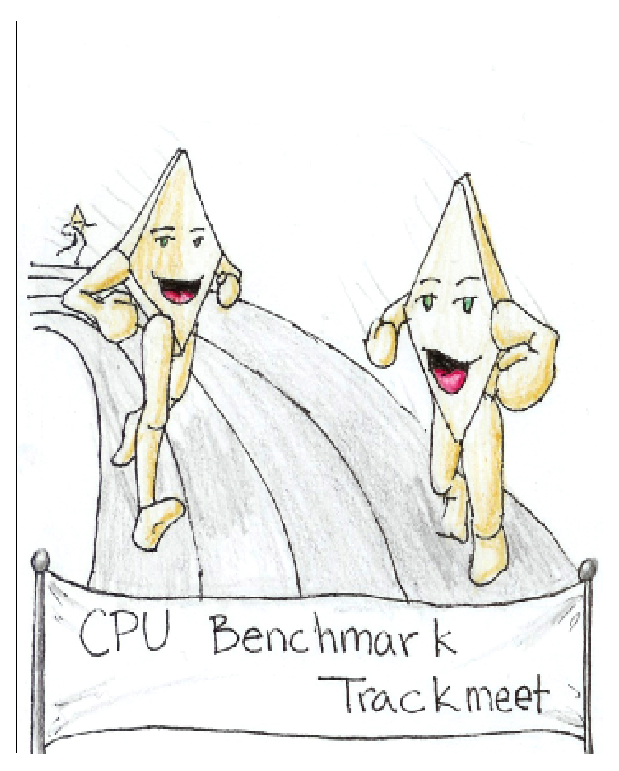
\includegraphics{cartoons/trackmeet}}
\end{center}
\caption{CPU Performance at its Best}
\label{fig:intro:CPU Performance at its Best}
\end{figure}

Although there are a few CPU-bound benchmarks that approach the ideal
shown in Figure~\ref{fig:intro:CPU Performance at its Best},
the typical program more closely resembles an obstacle course than
a race track.
This is because the internal architecture of CPUs has changed dramatically
over the past few decades, courtesy of Moore's Law.
In the early 1980s, the typical microprocessor fetched an instruction,
decoded it, and executed it, typically taking \emph{at least} three
clock cycles to complete one instruction before proceeding to the next.
In contrast, the CPU of the late 1990s and early 2000s will be executing
many instructions simultaneously, using a deep ``pipeline'' to control
the flow of instructions internally to the CPU, this difference being
illustrated by Figure~\ref{fig:intro:CPUs Old and New}.

\begin{figure}[htb]
\begin{center}
\resizebox{3in}{!}{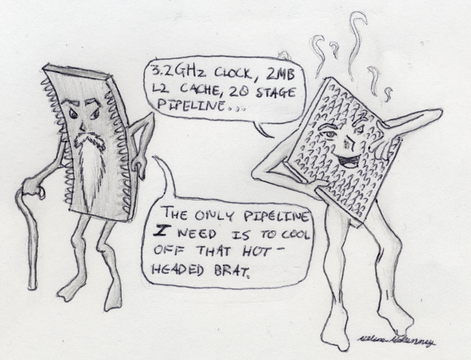
\includegraphics{cartoons/OldManAndBrat}}
\end{center}
\caption{CPUs Old and New}
\label{fig:intro:CPUs Old and New}
\end{figure}

\emph{@@@ check up on better .eps for figure.  Also insert block diagram
of CPU.}

Achieving full performance with a CPU having a long pipeline requires
highly predictable control flow through the program.
Suitable control flow can be provided by a program that executes primarily
in tight loops, for example, programs doing arithmetic on large matrices
or vectors.
The CPU can then correctly predict that the branch at the end of the loop
will be taken in almost all cases.
In such programs, the pipeline can be kept full and the CPU can execute
at full speed.

If, on the other hand, the program has many loops with small loop counts,
or if the program is object oriented with many virtual objects that
can reference many different real objects, all with different implementations
for frequently invoked member functions, then it is difficult or even
impossible for the CPU to predict where a given branch might lead.
The CPU must then either stall waiting for execution to proceed far enough
to know for certain where the branch will lead, or guess --- and, in
face of programs with unpredictable control flow, frequently guess wrong.
In either case, the pipeline will empty and have to be refilled, leading
to stalls that can drastically reduce performance,
as fancifully depicted in Figure~\ref{fig:intro:CPU Meets a Pipeline Flush}.

\begin{figure}[htb]
\begin{center}
\resizebox{3in}{!}{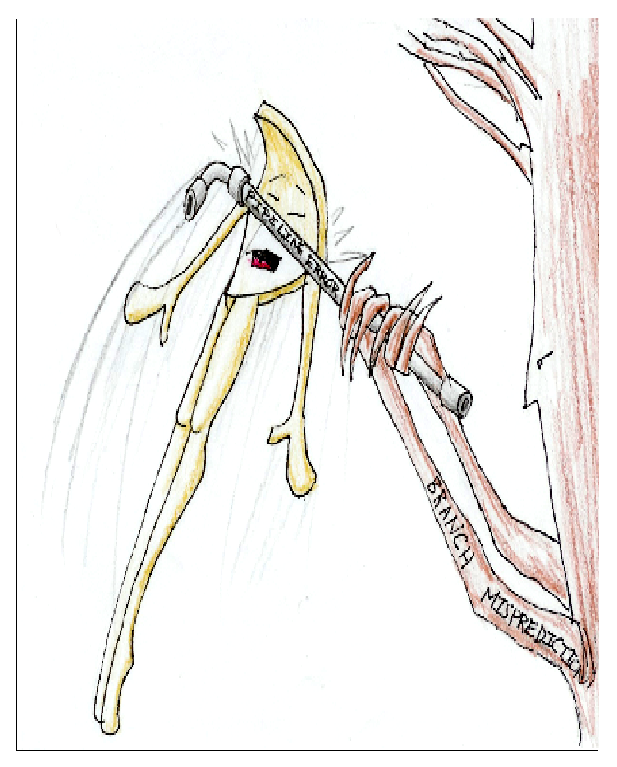
\includegraphics{cartoons/pipeline}}
\end{center}
\caption{CPU Meets a Pipeline Flush}
\label{fig:intro:CPU Meets a Pipeline Flush}
\end{figure}

Unfortunately, pipeline flushes are not the only hazards in the obstacle
course that modern CPUs must run.
In the 1980s, it often took less time for a microprocessor to load a value
from memory than it did to execute an instruction.
In 2006, a microprocessor might be capable of executing hundreds or even
thousands of instructions in the time required to access memory.
This disparity is due to the fact that Moore's Law has increased CPU
performance at a much greater rate than it has increased memory
performance, in part due to the rate at which memory sizes have
grown.\footnote{
	A typical 1980 computer might have 64KB (yes, kilobytes,
	not megabytes, let along gigabytes) of main memory.
	In 2006, CPU designers really can construct a 64KB memory
	with single-cycle access.
	And in fact they do, but it is now called a ``cache''.}

Although the large caches found on modern microprocessors can do quite
a bit to combat memory-access latencies,
just as keeping pipelines full requires highly predictable control flow,
these caches require highly predictable data-access patterns to
successfully hide memory latencies.
Unfortunately, common operations, such as traversing a linked list,
have extremely unpredictable memory-access patterns --- after all,
if the pattern was predictable, us software types would not bother
with the pointers, right?

Therefore, as shown in
Figure~\ref{fig:intro:CPU Meets a Memory Reference},
memory references are often severe obstacles for modern CPUs.

\begin{figure}[htb]
\begin{center}
\resizebox{3in}{!}{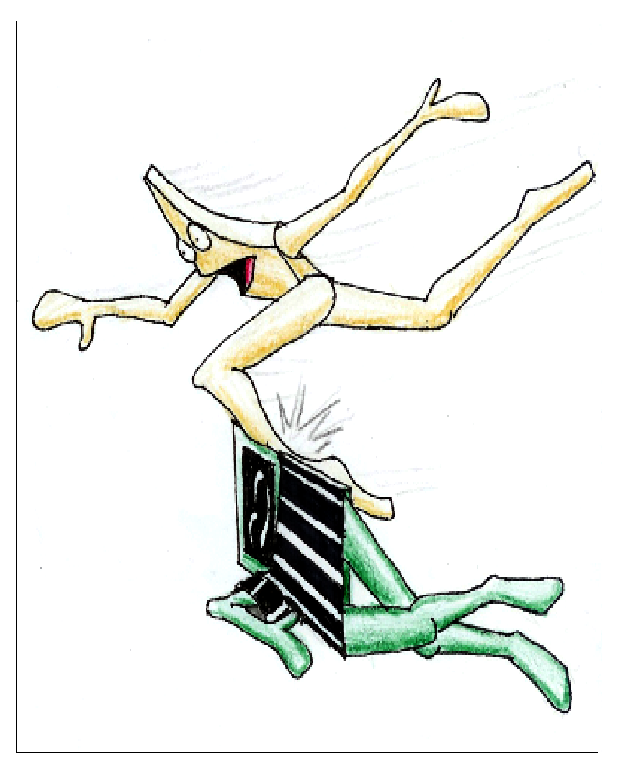
\includegraphics{cartoons/ref}}
\end{center}
\caption{CPU Meets a Memory Reference}
\label{fig:intro:CPU Meets a Memory Reference}
\end{figure}

Thus far, we have only been considering obstacles that can arise during
a given CPU's execution of single-threaded code.
Multi-threading presents additional obstacles to the CPU.

One such obstacle is atomic operations.
The whole idea of an atomic operation in some sense conflicts with
the piece-at-a-time assembly-line operation of a CPU pipeline.
To hardware designers' credit, modern CPUs use a number of very clever
tricks to make such operations \emph{look} atomic even though they
are in fact being executed piece-at-a-time, but even so, there are
cases where the pipeline must be delayed or even flushed in order to
permit a given atomic operation to complete correctly.

The resulting effect on performance is depicted in
Figure~\ref{fig:intro:CPU Meets an Atomic Operation}.

\begin{figure}[htb]
\begin{center}
\resizebox{3in}{!}{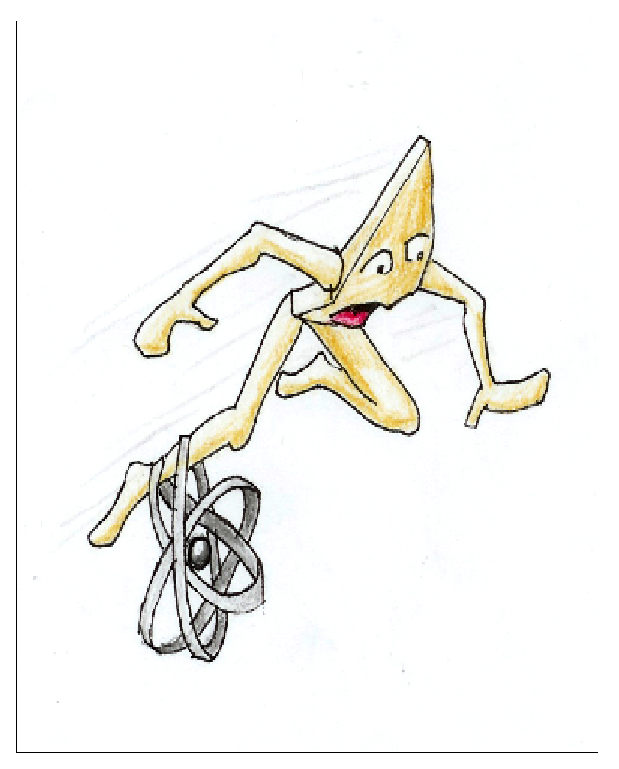
\includegraphics{cartoons/atomic}}
\end{center}
\caption{CPU Meets an Atomic Operation}
\label{fig:intro:CPU Meets an Atomic Operation}
\end{figure}

Another multi-threading obstacle to CPU performance stems from the
need of concurrent algorithms to maintain proper ordering of their
operations, as will be discussed in more detail in
Section~\ref{sec:advsync:Memory Barriers} and
Appendix~\ref{chp:app:whymb:Why Memory Barriers?}.
In the meantime, consider the following simple lock-based critical
section:

\vspace{5pt}
\begin{minipage}[t]{\columnwidth}
\small
\begin{verbatim}
  1 spin_lock(&mylock);
  2 a = a + 1;
  3 spin_unlock(&mylock);
\end{verbatim}
\end{minipage}
\vspace{5pt}

If the CPU were not constrained to execute these statements in the
order shown, the effect would be that the variable ``a'' would be
incremented without the protection of ``mylock'', which would certainly
defeat the purpose of acquiring it.
To prevent such destructive reordering, locking primitives contain
either explicit or implicit memory barriers.
Because the whole purpose of these memory barriers is to prevent reorderings
that the CPU would otherwise undertake in order to increase performance,
memory barriers almost always reduce performance, as depicted in
Figure~\ref{fig:intro:CPU Meets a Memory Barrier}.

\begin{figure}[htb]
\begin{center}
\resizebox{3in}{!}{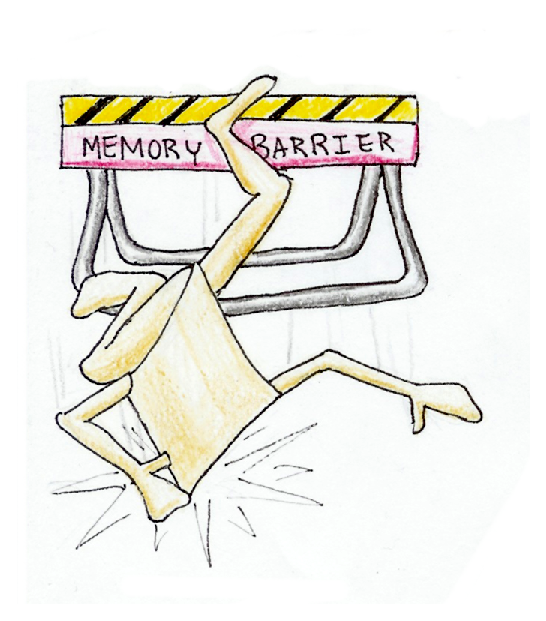
\includegraphics{cartoons/barrier}}
\end{center}
\caption{CPU Meets a Memory Barrier}
\label{fig:intro:CPU Meets a Memory Barrier}
\end{figure}

The final multi-threading obstacle to CPU performance is the ``cache miss''.
As noted earlier, modern CPUs sport large caches in order to reduce the
performance penalty that would otherwise be incurred due to slow memory
latencies.
However, these caches are actually counter-productive for variables that
are frequently shared among CPUs.
This is because when a given CPU wishes to modify the variable, it is
most likely the case that some other CPU has modified it recently.
In this case, the variable will be in that other CPU's cache, but not
in this CPU's cache, which will therefore incur an expensive cache miss
(see Section~\ref{sec:app:whymb:Cache Structure} for more detail).
Such cache misses form a major obstacle to CPU performance, as shown
in Figure~\ref{fig:intro:CPU Meets a Cache Miss}.

\begin{figure}[htb]
\begin{center}
\resizebox{3in}{!}{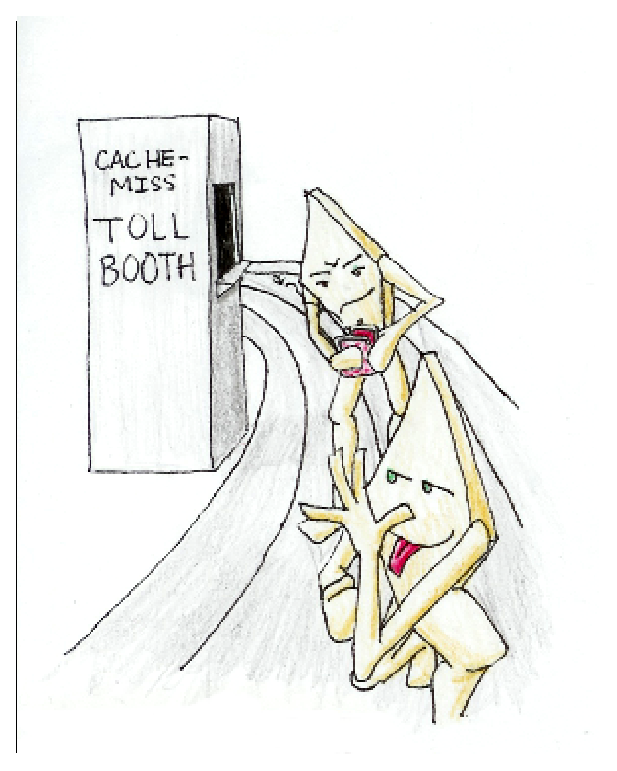
\includegraphics{cartoons/tollbooth}}
\end{center}
\caption{CPU Meets a Cache Miss}
\label{fig:intro:CPU Meets a Cache Miss}
\end{figure}

These obstacles can easily prevent your program from attaining its
potential on today's multi-core and multi-threaded hardware,
in fact, as we will see in Chapter~\ref{cha:SMP Synchronization Design}.
Much of the remainder of this book is dedicated to presenting
design rules, algorithms, and techniques that can help you
overcome these obstacles.
